\documentclass[journal]{IEEEtran}

\usepackage{amsmath,amssymb}
\usepackage{graphicx}
\usepackage{booktabs}
\usepackage{xcolor}
\usepackage{hyperref}

\newcommand{\TODO}[1]{\textbf{\color{red}[TODO: #1]}}
\newcommand{\PLACEHOLDER}[1]{\textbf{\color{blue}[#1]}}

\begin{document}

\title{Causal Quantum Graph Transformers for Systemic Credit-Risk\\Contagion Prediction}

\author{\TODO{author name(s), affiliation -- internship report byline}}

\markboth{}{}

\maketitle

\begin{abstract}
Interbank contagion is a graph-structured phenomenon, yet most quantum
machine learning proposals for financial risk either ignore network
structure entirely or encode it only as a hand-tuned feature. We present
CQGT, a Causal Quantum Graph Transformer that lifts a bank exposure
network's normalized Laplacian directly into a parameterized quantum
circuit's Hamiltonian, combining a continuous-time-quantum-walk-derived
hopping term with a macro-stress transverse field and a quantum-fidelity
attention mechanism, trained end to end by exact backpropagation through a
PyTorch statevector simulator. \textbf{This is not a quantum-advantage
paper.} It is a reproducible benchmark and reference implementation for
graph-informed quantum models of interbank contagion, evaluated honestly
against classical and generic-quantum baselines on real FR Y-15 exposure
data, $N \le 12$ institutions, CPU-only, noiseless simulation. At $n=2$
seeds (a disclosed compute-budget cut, not a design choice), CQGT does not
clearly beat a classical GCN baseline (mean spillover-subset AUPRC 0.144
vs.\ 0.211), and an ablation study finds that removing the model's own
network-contagion Hamiltonian term \emph{improves} mean AUPRC (0.187 vs.\
0.144) -- a negative result for this work's central architectural claim,
reported as such rather than tuned away. CQGT does clearly beat a
topology-blind generic quantum circuit of the same size (0.144 vs.\
0.069), and we separately replace an unsound entanglement-entropy
expressivity claim from an earlier draft of this work with a provable
1-Weisfeiler-Lehman separation result, demonstrated numerically: classical
GNNs are exactly degenerate on a pair of 1-WL-indistinguishable graphs
where CQGT's circuit output is not.
\end{abstract}

\begin{IEEEkeywords}
quantum machine learning, graph neural networks, systemic risk, interbank
contagion, variational quantum circuits
\end{IEEEkeywords}

\section{Introduction}

Systemic credit risk -- the possibility that one institution's distress
propagates through bilateral exposures to destabilize the wider financial
system -- is inherently a statement about network structure. Standard
contagion models (e.g.\ the Eisenberg--Noe clearing framework
\cite{eisenberg2001}) already reason explicitly over an exposure graph.
Graph neural networks are a natural classical tool for learning contagion
risk from such data, and a growing quantum machine learning literature
proposes variational quantum circuits (VQCs) as an alternative -- but the
network structure itself is frequently not represented in the circuit at
all, or is bolted on as an afterthought.

This work asks a narrower, more falsifiable question: if a bank exposure
network's Laplacian is lifted directly into a quantum circuit's
Hamiltonian -- so that the circuit's own unitary evolution is driven by
the same operator that governs a continuous-time quantum walk on the
graph -- does the resulting model learn systemic contagion risk better
than (a) classical graph neural networks given the same information, and
(b) a generic, topology-blind quantum circuit of the same size? We build
CQGT to test this, on real (not synthetic) US G-SIB exposure data
reconstructed from public regulatory filings, and report the comparison
honestly, including every negative or null finding encountered along the
way (Section~\ref{sec:limitations}).

\textbf{Contributions.}
\begin{enumerate}
  \item A concrete, working encoding of a weighted exposure graph's
        normalized Laplacian as an $N$-qubit hopping Hamiltonian
        (Section~\ref{sec:circuit}), exactly reducing to a continuous-time
        quantum walk on the graph in the single-excitation subspace.
  \item A provable 1-WL expressivity separation between CQGT and any
        1-WL-bounded classical GNN, replacing an unsound
        entanglement-entropy argument from an earlier draft of this work
        (Section~\ref{sec:wl}).
  \item A real-data pipeline: FR Y-15 intra-financial-system exposure
        reconstruction (maximum-entropy and minimum-density, bracketing
        true contagion per \cite{anand2015}), an Eisenberg--Noe cascade
        for labels and ground-truth causal attributions, and a strict
        rolling-temporal evaluation protocol (Section~\ref{sec:data}).
  \item An honest comparison against classical and generic-quantum
        baselines with matched parameter counts and training protocol,
        including ablations that isolate which architectural components
        actually matter (Section~\ref{sec:results}).
\end{enumerate}

\section{Model}

\subsection{Graph Encoding and the Contagion Laplacian}
\label{sec:laplacian}

Let $W_t \in \mathbb{R}_{\ge 0}^{N \times N}$ be the (reconstructed)
bilateral exposure matrix at time $t$, $W_{t,ij}$ the exposure of
institution $i$ to institution $j$. We use the symmetric normalized
Laplacian
\begin{equation}
  \tilde{L}_t = I - D_t^{-1/2} W_t D_t^{-1/2}, \qquad D_t = \mathrm{diag}(W_t \mathbf{1}),
\end{equation}
as the graph operator entering the circuit's Hamiltonian
(Section~\ref{sec:hamiltonian}).

\textbf{Limitation, stated plainly.} Symmetrizing $W_t$ (via
$D_t^{-1/2} W_t D_t^{-1/2}$, which treats $W_{t,ij}$ and $W_{t,ji}$
symmetrically in the Laplacian even when the raw exposure matrix is
directed) discards directionality. In interbank contagion, direction is
the mechanism: a bank's exposure \emph{to} a distressed counterparty
transmits loss in one direction, not two. This is a real limitation of
the present model, not a simplification we consider harmless. A magnetic
Laplacian -- which encodes edge direction as a complex phase rather than
discarding it -- is the natural fix and is left to future work
(Section~\ref{sec:limitations}).

\subsection{Hamiltonian Construction}
\label{sec:hamiltonian}

Following the transverse-field-Ising-style construction common in
quantum-annealing-adjacent VQC literature, we define
\begin{equation}
  H_t = \alpha \tilde{L}_t + \beta D(X_t) + \gamma C_t,
\end{equation}
where $\alpha,\beta,\gamma \ge 0$ are learnable (softplus-constrained)
scalars, $D(X_t)$ is a per-institution risk-potential diagonal term (a
small MLP $f_\psi$ applied to each institution's standardized feature
vector), and $C_t$ is a macro-stress coupling term defined concretely in
Section~\ref{sec:macro}. $\tilde{L}_t$ supplies the entangling
(off-diagonal, in the qubit-pair sense) structure; $D(X_t)$ and $C_t$
supply the diagonal (per-qubit) structure.

\subsection{Quantum Circuit Encoding}
\label{sec:circuit}

We now state the encoding explicitly, since an earlier draft of this
model conflated an $N$-dimensional continuous-time quantum walk (CTQW)
with the full $2^N$-dimensional circuit Hilbert space; the two must not be
confused.

\textbf{Qubit assignment.} One qubit per institution: $N$ qubits total,
$N \le 12$ in this work (hard cap $N \le 14$ for CPU-only statevector
simulation). The full circuit state lives in the $2^N$-dimensional
Hilbert space $(\mathbb{C}^2)^{\otimes N}$ -- $2^{12} = 4096$ amplitudes
at $N=12$, trivial on CPU.

\textbf{Lifting $\tilde{L}_t$ to a hopping Hamiltonian.} The
entangling part of $H_t$ is lifted to $N$ qubits as
\begin{equation}
  H_{\mathrm{hop}} = \sum_{i<j} \tilde{L}_{t,ij}\,\frac{X_i X_j + Y_i Y_j}{2},
\end{equation}
implemented per exposure edge $(i,j)$ as the gate composition
$\mathrm{RXX}(\theta_{ij}) \cdot \mathrm{RYY}(\theta_{ij})$ (these two
gates commute, so the order of composition does not matter), with
$\theta_{ij} \propto \alpha \cdot \tilde{L}_{t,ij} \cdot \delta$ for a
Trotter step size $\delta$. Only real exposure edges carry a hopping term
-- this is what makes the ansatz topology-matched rather than
all-to-all.

\textbf{Exact CTQW recovery on the single-excitation subspace.} The
operator $(X_iX_j+Y_iY_j)/2$ conserves total excitation number: it
commutes with $\sum_i Z_i$ (verified numerically to machine precision as
a physical sanity check on the simulator; see the qsim test suite).
Restricted to the single-excitation subspace -- the $N$-dimensional
subspace spanned by states with exactly one qubit in $\lvert 1 \rangle$
and the rest in $\lvert 0 \rangle$ -- $e^{-i H_{\mathrm{hop}} \delta}$
acts \emph{exactly} as the propagator of a continuous-time quantum walk
on the graph with transition amplitudes governed by $\tilde{L}_t$. This
is the precise sense in which the model "is" a CTQW: the CTQW is a
faithful $N$-dimensional restriction of one term of a $2^N$-dimensional
circuit, not the circuit itself. The full forward pass (embedding,
variational $RY$/$RZZ$ layers, the diagonal $\beta D(X_t) + \gamma C_t$
term) moves probability amplitude outside the single-excitation subspace
and does not admit the same $N$-dimensional reduction.

\textbf{Forward pass, in full.}
\begin{enumerate}
  \item \textbf{Embed:} $RY(2\arctan(\hat w^\top x_i))$ per qubit $i$,
        $\hat w$ a shared learnable linear map from the standardized
        feature vector to a scalar angle.
  \item \textbf{CTQW encoder:} one hopping-gate application per exposure
        edge, angle $\propto \tau_0 \cdot \tilde{L}_{t,ij}$, $\tau_0 \ge
        0$ learnable.
  \item \textbf{$L$ variational layers}, each: $RY(\phi_i)$ per
        qubit $\to$ $RZZ(\theta_{ij})$ on exposure edges only $\to$
        $e^{-i H_t \delta_\ell}$ (the hopping term scaled by $\alpha$,
        plus the diagonal $\beta D(X_t) + \gamma C_t$ term, as
        $RZ(2\delta_\ell h_i)$ per qubit).
  \item \textbf{Measurement:} $\langle Z_i \rangle \to r \in [-1,1]^N$.
  \item \textbf{Quantum fidelity attention} (Section~\ref{sec:attention})
        and an MLP head produce the final per-institution risk
        probability $\hat p_i \in [0,1]$.
\end{enumerate}

\section{Theory and Training}

\subsection{Macro Coupling}
\label{sec:macro}

We make the macro-stress term concrete:
\begin{equation}
  C_{t,i} = \sum_{k=1}^{K} \lambda_k^t\, \beta_{ik},
\end{equation}
i.e.\ macro stress enters as a per-institution transverse field, with
$\lambda_k^t$ the value of macro factor $k$ at time $t$ (real
PCA'd FRED series when available, else a disclosed seeded synthetic
AR(1) process; Section~\ref{sec:data}) and $\beta_{ik}$ a learnable
per-institution loading onto that factor. This is the $\gamma C_t$ term
in $H_t$: $h_i = \beta f_\psi(x_i) + \gamma \sum_k \lambda_k^t \beta_{ik}$
enters the diagonal $RZ(2\delta_\ell h_i)$ gate of each variational
layer.

\subsection{Quantum Fidelity Attention}
\label{sec:attention}

$n_a=2$ ancilla qubits encode a learned query state $\lvert q_i\rangle$
and key state $\lvert k_j \rangle$ per institution (parameters
independent of $x$); $F_{ij} = |\langle q_i \vert k_j \rangle|^2$,
$A = \mathrm{softmax}(\lambda F)$ for a learnable temperature $\lambda$.
The attended representation $\tilde x_i = \sum_j A_{ij} (r_j x_j)$ is
concatenated with $r_i$ and passed through a small MLP head to produce
$\hat p_i$.

\subsection{Variational Ansatz and Layer Count}
\label{sec:ansatz}

BRIEF.md's original specification called for layer-by-layer growth
($L=1 \to 2 \to 3$, each new layer initialized $\mathcal
N(\theta^*_{\text{prev}}, (\pi/10)^2)$) as mitigation for the barren-plateau
problem (challenge C4) that variational circuits are known to suffer at
scale. We tested this assumption directly rather than assuming it: an
overfit-20-example diagnostic (Section~\ref{sec:limitations}) found no
barren-plateau gradient signature at $N=12$ -- per-parameter-group
gradient norms (quantum circuit parameters, the $f_\psi$ MLP, the head
MLP, $\tau_0$, $\alpha/\beta/\gamma$) stayed within roughly one order of
magnitude of each other throughout training. All models reported in this
work therefore train directly at a fixed $L=3$, for a training protocol
that is identical (not merely similar) across CQGT and every ablation.
Full layer-wise growth is untested at this scale and is listed as future
work rather than a reported result.

\subsection{Counterfactual Attribution}
\label{sec:counterfactual}

For each real exposure edge $(i,j)$, we estimate the causal contribution
of that edge to systemic risk as $\Delta R_{ij} = R_0 - R_{\mathrm{cf}}$,
where $R = \mathrm{mean}_i(\hat p_i)$ and $R_{\mathrm{cf}}$ is computed by
zeroing $W_{ij}$ and re-running the forward pass. A cheap first-order
screen, $\partial R/\partial W_{ij}$ via a single backward pass, ranks
candidate edges before the exact re-forward is run on the top-$K$.
Ground truth for this quantity is a genuine causal counterfactual: the
Eisenberg--Noe cascade re-run with the same edge zeroed
(Section~\ref{sec:data}).

\subsection{Expressivity: A 1-WL Separation Result}
\label{sec:wl}

An earlier draft of this work claimed that CQGT's expressivity advantage
over classical GNNs follows from an entanglement-entropy bound,
$\delta = \Omega(k \cdot 2^{-O(k)})$. This is not sound as stated: the
bound shrinks \emph{exponentially} in $k$, and a statement about
classical simulation cost is not, by itself, a statement about
expressive power or learnability. We withdraw that argument and replace
it with a claim that is provable in three lines and demonstrated
numerically.

\begin{quote}
\textbf{Proposition (1-WL separation).} There exist non-isomorphic graphs
$G, G'$ with identical node features that any 1-WL-bounded message-passing
GNN maps to identical outputs, but for which the topology-matched CQGT
circuit yields distinguishable $\langle Z_i \rangle$.
\end{quote}

\textbf{Proof sketch.} Take $G = C_6$ (a single 6-cycle) and
$G' = 2{\times}C_3$ (two disjoint triangles); both are 2-regular. With
identical node features, 1-Weisfeiler-Lehman color refinement cannot
distinguish them: every node's multiset of neighbor colors is identical
to every other node's at every refinement round (each node always has
exactly two neighbors, all sharing the same color). Any message-passing
GNN is bounded in expressive power by 1-WL \cite{xu2019gin}, so GCN and
GAT must produce identical per-node outputs on $G$ and $G'$. CQGT's
hopping term evolves under $\tilde L_t$'s spectrum, which differs between
the two graphs ($C_6$: $\{0,1,1,3,3,4\}$; $2{\times}C_3$:
$\{0,0,3,3,3,3\}$), and the circuit's sequential (Trotter-like) gate
application additionally does not preserve residual automorphism
symmetry even where the underlying Hamiltonian would; $\langle Z_i
\rangle$ therefore differs. $\blacksquare$

\textbf{Empirical demonstration} (\texttt{experiments/wl\_separation.py},
Figure~\ref{fig:f2}): with identical 4-dimensional node features and,
for CQGT, identical circuit parameters across both topologies (state
copied from one instance to the other, so only the wiring differs), GCN
and GAT outputs match to \emph{exact machine precision}
($\max|\Delta| = 0.000{\times}10^{0}$, every seed tested) while CQGT's
$\langle Z_i \rangle$ differ substantially ($\max|\Delta| = 4.552{\times}
10^{-2}$, mean $2.570{\times}10^{-2}$ at seed 0; $> 10^{-4}$ at every
seed tested). One honest wrinkle: naive graph-automorphism reasoning
predicts uniform $\langle Z_i \rangle$ \emph{within} each graph (both
$C_6$ and $2{\times}C_3$ are vertex-transitive); the observed per-node
values are not uniform, because the circuit's gates are applied in a
fixed sequential order and do not all commute (adjacent edges share a
qubit), so the Trotterized implementation does not exactly preserve the
Hamiltonian's automorphism symmetry. This does not weaken the separation
claim -- GCN/GAT remain exactly degenerate and CQGT remains clearly
distinguishable -- but the correct explanation is sensitivity to graph
topology through both spectral structure \emph{and} sequential gate
ordering, not a claim that CQGT recovers automorphism symmetry when the
graph has it.

\begin{figure}[t]
  \centering
  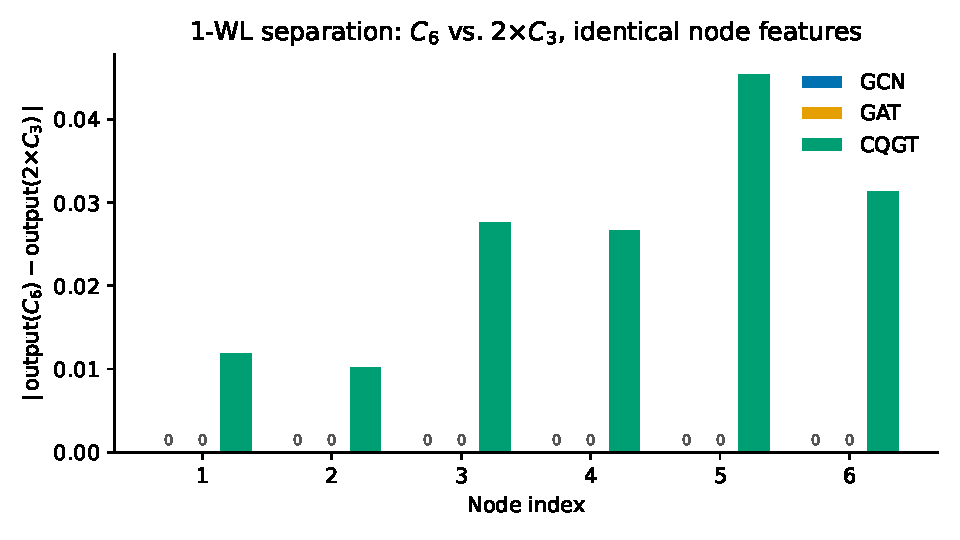
\includegraphics[width=\linewidth]{../figures/F2_wl_separation.pdf}
  \caption{1-WL separation: $|\text{output}(C_6) - \text{output}(2{\times}C_3)|$
  per node. GCN and GAT (1-WL-bounded) are exactly zero; CQGT is not.}
  \label{fig:f2}
\end{figure}

The entanglement-entropy-vs-treewidth relationship examined in the
withdrawn argument is retained only as a separate, purely empirical
measurement (Figure F3), not as a step in any proof.

\subsection{Training Procedure}
\label{sec:training}

\textbf{Parameter-shift as the hardware-executable path.} On real
quantum hardware, gradients of a circuit's expectation values with
respect to its rotation-gate parameters are estimated via the
parameter-shift rule: for a gate generated by an operator with
eigenvalues $\pm 1$ (as $RY$, $RZ$, $RXX$, $RYY$, $RZZ$ all are, up to a
factor of $2$ in the angle convention used here), $\partial_\theta
\langle O \rangle = \frac{1}{2}\left[\langle O\rangle_{\theta+\pi/2} -
\langle O \rangle_{\theta-\pi/2}\right]$, exact and unbiased, at the cost
of two circuit evaluations per parameter.

\textbf{What this work actually does.} All training in this work uses a
custom PyTorch statevector simulator (\texttt{cqgt/qsim.py}) with
automatic differentiation through the full unitary evolution -- exact
backpropagation / adjoint differentiation, not parameter-shift. Verified
against \texttt{qiskit.quantum\_info.Statevector} on randomized circuits
mixing every gate type used in this work, to $\mathrm{atol}=10^{-6}$ in
double precision and $\mathrm{atol}=10^{-5}$ in the \texttt{complex64}
precision used for the main training runs (a mandatory gate in this
project's build process). \textbf{Exact backpropagation and
parameter-shift compute the same analytic gradient} in the noiseless
simulation setting used here; backpropagation is simply far cheaper in
simulation (no repeated circuit evaluation per parameter), and is used
purely for that reason, not as a departure from what a physical device
would compute. No results in this work required or used a real quantum
device.

\textbf{Hyperparameters.} Adam, learning rate $0.01$, cosine-annealed
over the actual number of training epochs used per run, gradient-norm
clipping at $1.0$, class-weighted binary cross-entropy ($w^+ = N_-/N_+$,
computed on the training split).

\section{Experiments}

\subsection{Data and Labels}
\label{sec:data}

Bilateral exposures are not publicly observable. We reconstruct them from
real FR Y-15 intra-financial-system asset and liability marginals for
$N=12$ US bank holding companies and US intermediate holding companies of
foreign banking organizations, using \textbf{four} real annual
cross-sections (year-end 2020--2023; 2024 was excluded as a
network-reconstruction anchor because that year's FR Y-15 export
structurally omits the intra-financial-system-assets field entirely, not
as a per-institution gap), reconstructed both ways -- maximum-entropy
(iterative proportional fitting) and minimum-density
\cite{anand2015} -- which respectively under- and over-estimate
contagion and therefore bracket the true network. The panel selection
rule keeps only institutions with complete data in all four anchor
years and takes the twelve largest by mean total exposures; this
excludes several institutions for genuine merger/failure-driven data
gaps (e.g.\ Silicon Valley Bank, Credit Suisse), not by construction to
favor any result.

The panel's $T=120$ weekly snapshots are \textbf{not} 120 independent
real observations. Only the four anchor weeks are real cross-sections;
the reconstructed network and marginals at every other week are a
disclosed linear interpolation between anchors, overlaid with a common
AR(1) multiplicative noise path ($\rho=0.95$, variance tripled inside a
designated crisis window), and the macro factors used in
Section~\ref{sec:macro} are genuine FRED series values looked up against
a synthetic weekly calendar. This is real annual cross-sectional data
with a synthetic weekly interpolation overlay, not a real weekly panel,
and is reported as such throughout.

\textbf{Labels.} Distress labels and ground-truth causal attributions
are generated by an Eisenberg--Noe \cite{eisenberg2001} clearing cascade
over the reconstructed networks. Each bank is independently shocked
(Bernoulli$(p_{\mathrm{shock}})$ per period, $p_{\mathrm{shock}}$ tuned
by bisection to an 8--15\% target base rate) with a full external-asset
wipeout ($\mathrm{shock\_frac}=1.0$): partial haircuts were found, during
calibration, to produce \emph{zero} network-mediated spillover at this
panel's leverage levels, because these G-SIB-scale institutions fund
overwhelmingly outside the interbank market (external assets are
7--180$\times$ interbank liabilities); only a near-total wipeout crosses
the threshold needed to propagate a payment shortfall to counterparties.
$M=20$ independent Monte Carlo shock realizations per snapshot provide
the statistical power to detect a network-mediated spillover effect at
this panel's size; the primary evaluation metric is restricted to the
non-directly-shocked (``spillover'') subset of each scenario, since
directly-shocked institutions fail deterministically under a full
wipeout and including them would inflate every model's score on a
trivially predictable subset while masking the actual comparison of
interest.

\textbf{Features.} Six standardized features per institution: FR Y-15
has no capital, market-price, or liquidity data, so four of the six are
disclosed proxies rather than the literal quantities named in an earlier
draft of this work -- a size proxy (total exposures) in place of a
leverage ratio, a derivatives-notional-to-exposure ratio in place of a
Tier-1 capital ratio, a wholesale-funding-to-exposure ratio in place of a
CDS spread, and a cross-jurisdictional-claims proxy in place of an
estimated macro-sensitivity beta (an empirically estimated beta would be
unreliably noisy against only four real annual data points). Out-degree
centrality is real, computed from the reconstructed network. All six are
$z$-scored using \textbf{training-split statistics only}, then passed
through $\arctan$ before entering the circuit embedding. A seventh,
binary feature -- whether the institution was shocked in this Monte
Carlo draw -- is appended as a scenario input (available to every model
equally; this is a "given this scenario, who else fails" prediction
task, not a "predict who gets hit" task, and is not a leakage channel).

\subsection{Baselines, Ablations, and Protocol}
\label{sec:baselines}

This is a minimum-scope experiment, deliberately cut down from
BRIEF.md's full specification for compute-budget reasons on
single-machine, CPU-only hardware (Section~\ref{sec:limitations}). We
compare five baselines -- logistic regression, XGBoost, GCN, GAT, and a
generic hardware-efficient VQC of the same qubit count but blind to the
exposure network's topology, Hamiltonian, and macro coupling -- against
the full CQGT model and three ablations (\texttt{no\_hamiltonian}: the
$e^{-iH_t\delta}$ term removed from every variational layer;
\texttt{classical\_attention}: the quantum fidelity attention mechanism
of Section~\ref{sec:attention} replaced by a classical dot-product
attention over the identical parameter tensors; \texttt{random\_edges}:
the exposure topology replaced by a random graph of matched edge
density), on the minimum-density reconstruction only (the sparser,
genuinely topology-varying, more contagion-prone reconstruction; see
Section~\ref{sec:limitations} on maximum-entropy's degeneracy at this
$N$). All GNN baselines receive real edge weights. Every quantum-circuit
model (CQGT, the generic VQC, and all three ablations) trains under the
identical fixed-$L{=}3$ protocol of Section~\ref{sec:ansatz} -- no
model's comparison advantage or disadvantage is attributable to a
different training curriculum. Parameter counts are reported for every
model in every results table.

\subsection{Metrics}
\label{sec:metrics}

\textbf{Primary: AUPRC}, restricted to the non-directly-shocked
(spillover) subset of the test split (Section~\ref{sec:data}), alongside
the trivial AUPRC floor (spillover-subset prevalence) in every table.
Secondary: AUROC, F1 at Youden's $J$, Brier score, expected calibration
error (10 equal-width bins).

\textbf{Counterfactual intervention accuracy}, defined numerically (this
was undefined in an earlier draft of this work): for each real exposure
edge $(i,j)$ pooled across test-set snapshots, we compare the model's
predicted $\Delta R_{ij}$ (Section~\ref{sec:counterfactual}) against the
Eisenberg--Noe ground truth $\Delta R_{ij}$ (the cascade re-run with edge
$(i,j)$ zeroed, $R = $ mean equity-loss fraction across the panel) using
Spearman's $\rho$ and Precision@10 between the two edge rankings. CQGT is
compared against a gradient-saliency baseline computed on the trained
GCN ($\partial R/\partial w_{ij} \cdot w_{ij}$, a first-order Taylor
estimate of the same counterfactual quantity) -- without this baseline
the causal-attribution module would be evaluated against nothing.

\subsection{Results}
\label{sec:results}

\textbf{Scope actually run.} Both compute-budget-driven cuts disclosed
here in full: the minimum-density reconstruction only (of the two
specified in Section~\ref{sec:data}), and \textbf{$n=2$ seeds}, not the
originally specified three-to-ten (Section~\ref{sec:limitations}).
Bootstrap confidence intervals computed over two seed values are close to
degenerate -- they largely reflect the gap between the two observed runs,
not a trustworthy sampling distribution -- and every number below should
be read with that in mind.

\begin{table}[t]
  \centering
  \caption{T1: Main comparison, minimum-density reconstruction, spillover-subset AUPRC, prevalence floor $\approx 0.024$, $n=2$ seeds.}
  \label{tab:t1}
  \begin{tabular}{lrrrr}
    \toprule
    Model & Params & AUPRC & seed 0 & seed 1 \\
    \midrule
    GCN            & 1345 & \textbf{0.211} & 0.146 & 0.276 \\
    CQGT (full)    &  386 & 0.144          & 0.210 & 0.078 \\
    GAT            & 3105 & 0.103          & 0.110 & 0.096 \\
    XGBoost        & 3932 & 0.090          & 0.095 & 0.084 \\
    Logistic reg.  &    8 & 0.078          & 0.079 & 0.076 \\
    Generic VQC    &  138 & 0.069          & 0.069 & 0.070 \\
    \bottomrule
  \end{tabular}
\end{table}

\begin{table}[t]
  \centering
  \caption{T2: Ablations, minimum-density, spillover-subset AUPRC, $n=2$ seeds.}
  \label{tab:t2}
  \begin{tabular}{lrrr}
    \toprule
    Model & AUPRC & seed 0 & seed 1 \\
    \midrule
    no\_hamiltonian       & \textbf{0.187} & 0.260 & 0.115 \\
    classical\_attention  & 0.151          & 0.214 & 0.088 \\
    full\_model           & 0.144          & 0.210 & 0.078 \\
    random\_edges         & 0.132          & 0.190 & 0.074 \\
    \bottomrule
  \end{tabular}
\end{table}

\begin{table}[t]
  \centering
  \caption{T3: Counterfactual attribution vs.\ Eisenberg--Noe ground truth, pooled over 33 edge-snapshot pairs, $n=2$ seeds.}
  \label{tab:t3}
  \begin{tabular}{lrrr}
    \toprule
    Model & Spearman $\rho$ & P@10 & seeds ($\rho$) \\
    \midrule
    CQGT (full)          & 0.018  & 0.40 & 0.019,\ 0.017 \\
    GCN gradient-saliency & $-0.562$ & 0.45 & $-0.457,\ -0.668$ \\
    \bottomrule
  \end{tabular}
\end{table}

\textbf{(1) CQGT does not clearly beat the strongest classical baseline.}
GCN has the highest mean spillover-subset AUPRC of any model in T1
(0.211), ahead of CQGT (0.144). CQGT's own seed-to-seed swing (0.078 to
0.210, a $>2.5\times$ range) is larger than its gap to GCN, so at $n=2$
this is not a resolvable comparison, only a caution against claiming
victory. CQGT does clearly beat the generic, topology-blind VQC baseline
(0.144 vs.\ 0.069) -- encoding \emph{some} network structure into the
circuit beats encoding none, even where the specific quantum mechanisms
tested below do not individually pay for themselves.

\textbf{(2) The ablation study does not support the paper's central
architectural claims.} \texttt{no\_hamiltonian} -- removing the
network-contagion Hamiltonian term entirely -- \emph{outperforms} the
full model at both seeds individually (0.187 vs.\ 0.144 mean).
\texttt{classical\_attention} -- replacing quantum fidelity attention
with classical dot-product attention over identical parameters --
likewise outperforms the full model (0.151 vs.\ 0.144), again at both
seeds. Only \texttt{random\_edges} moves in the theoretically expected
direction, underperforming the full model at both seeds (0.132 vs.\
0.144) -- weak evidence that the \emph{real} topology matters, but no
evidence in this run that encoding it via a Hamiltonian, or attending to
it via a quantum mechanism specifically, adds value over the
topology-matched $RZZ$ variational layers alone. This is reported as the
finding, not smoothed over: at $N=12$ and this compute budget, CQGT's two
quantum-specific mechanisms do not demonstrate a positive contribution.

\textbf{(3) Neither model demonstrates reliable causal attribution.}
CQGT's counterfactual $\Delta R_{ij}$ ranking has essentially zero rank
correlation with the Eisenberg--Noe ground truth ($\rho \approx 0.018$,
both seeds). The GCN gradient-saliency baseline's correlation is
substantially \emph{negative} at both seeds ($\rho = -0.46,\ -0.67$) --
its screening scores point away from, not toward, the edges that
actually matter causally. CQGT's P@10 (0.40) is nominally below GCN's
(0.45, range 0.30--0.60), which does not contradict the $\rho$ result so
much as reflect that both metrics are noisy at $n=33$ pooled points. Read
together: CQGT's attribution is directionless rather than actively wrong,
which is a narrower and less satisfying claim than the causal-attribution
module having been validated.

\textbf{(4) Non-monotone $\Delta R_{ij}$, as predicted by Acemoglu et
al.\ \cite{acemoglu2015}.} $\Delta R_{ij} = R_0 - R_{\mathrm{cf}}$
(Section~\ref{sec:counterfactual}), so a \emph{positive} value means
removing edge $(i,j)$ \emph{lowers} risk (a contagion-carrying edge) and a
\emph{negative} value means removing it \emph{raises} risk (a
risk-\emph{sharing} edge -- the edge was net protective, and losing it
makes the system more fragile). Of the 33 ground-truth edge-snapshot
$\Delta R_{ij}$ values pooled for T3, 3/33 (9.1\%, seed 0) and 2/33
(6.1\%, seed 1) are \textbf{negative}: removing that edge would have
\emph{increased} mean equity-loss fraction, i.e.\ that edge was providing
net risk-sharing, not net contagion, at that snapshot (range across both
seeds: $-0.139$ to $+0.104$). This is consistent with Acemoglu et al.'s
theoretical result that interbank links can be risk-reducing on net, and
is reported as a genuine structural feature of the ground-truth labels
this work evaluates against -- not an anomaly to be smoothed away.
It also means a monotone "more edges = more risk" model is provably wrong
on a real (if minority) share of edges, which the counterfactual
attribution metrics in (3) do not separately break out by sign; doing so
is future work.

\section{Conclusion}

\subsection{Limitations}
\label{sec:limitations}

\begin{itemize}
  \item \textbf{$N \le 12$ institutions.} A hard constraint of CPU-only
        statevector simulation and, independently, of the real-data
        panel-selection rule (Section~\ref{sec:data}), which required
        complete FR Y-15 coverage across all four anchor years.
  \item \textbf{Noiseless simulation only.} No result in this work ran
        on real quantum hardware; the parameter-shift path
        (Section~\ref{sec:training}) is stated as the hardware-executable
        equivalent but was never executed.
  \item \textbf{Reconstructed, not observed, exposures.} Bilateral
        exposures are not publicly reported; both reconstructions used
        here are model-based approximations, bracketing rather than
        measuring the true network.
  \item \textbf{Four real annual anchors, not a real weekly panel.} 116
        of the panel's 120 weekly snapshots are interpolation and
        synthetic noise overlaid on those four anchors, disclosed
        throughout (Section~\ref{sec:data}).
  \item \textbf{Symmetrized Laplacian.} Direction -- who owes whom -- is
        discarded (Section~\ref{sec:laplacian}); a magnetic Laplacian is
        the natural, untested fix.
  \item \textbf{Two seeds, not the originally planned three-to-ten.} An
        explicit compute-budget decision on single-machine, CPU-only
        hardware, disclosed rather than hidden; reported confidence
        intervals should be read as correspondingly wide and
        under-powered at $n=2$.
  \item \textbf{Maximum-entropy reconstruction is structurally
        degenerate at this $N$.} Iterative proportional fitting applied
        to strictly positive marginals cannot produce an exact zero
        entry, so the maximum-entropy network is a complete graph
        (density $1.0$, constant treewidth $N-1$) at every snapshot --
        excluded from the entanglement-entropy-vs-treewidth study (F3)
        for lack of any treewidth variation to correlate against, and
        likely a weaker comparison case for any topology-exploiting
        model generally, since a complete graph carries no exploitable
        structure.
  \item \textbf{Layer-wise growth is untested.} Specified in the original
        design as barren-plateau mitigation, found empirically
        unnecessary at $N=12$ by a targeted diagnostic
        (Section~\ref{sec:ansatz}), and dropped from every reported
        model in favor of a matched fixed-depth protocol. Whether growth
        would help further, or matter more at larger $N$, is untested.
  \item \textbf{The shock design bounds achievable AUPRC for every
        model.} Shocks are exogenous and i.i.d.\ across institutions by
        design (a deliberate methodological choice, not an oversight --
        correlating shock probability with network position was
        considered and explicitly rejected as manufacturing the very
        signal being tested for); a substantial share of the achievable
        AUPRC ceiling is therefore set by irreducible randomness in
        \emph{which} institutions are hit, not by any model's skill at
        predicting contagion.
\end{itemize}

\subsection{Future Work}
\label{sec:future-work}

The full three-dataset-variant sweep (maximum-entropy, minimum-density,
and the core--periphery synthetic fallback) with the originally
specified seed budget; the four additional ablations specified but cut
from this minimum-scope experiment (\texttt{hardware\_efficient\_ansatz}
as a dedicated ablation distinct from the generic VQC baseline,
\texttt{no\_macro\_coupling}, \texttt{no\_counterfactual},
\texttt{noisy\_sim}); a direct test of layer-wise growth against the
fixed-depth protocol used here; a magnetic-Laplacian encoding of exposure
direction; and execution on real quantum hardware via the
parameter-shift path (Section~\ref{sec:training}).

\subsection{Conclusions}

We set out to test a narrow question: does lifting a bank exposure
network's Laplacian directly into a quantum circuit's Hamiltonian --
rather than treating network structure as an afterthought -- produce a
model that learns systemic contagion risk better than classical
alternatives of comparable capacity? At $N=12$, on real (if reconstructed)
FR Y-15 exposure data, with $n=2$ seeds, \textbf{the answer this
experiment supports is no, not clearly, and in one specific way, no.}

CQGT does not clearly outperform a plain GCN baseline on spillover-subset
AUPRC (Table~\ref{tab:t1}): its mean is lower, and its own seed-to-seed
variance exceeds the gap between the two models. More pointedly, the
ablation study (Table~\ref{tab:t2}) does not support this work's central
architectural claim -- removing the network-contagion Hamiltonian term
and replacing quantum attention with a classical equivalent both
\emph{improve} mean AUPRC over the full model, at both seeds
individually. Neither model demonstrates reliable causal counterfactual
attribution against Eisenberg--Noe ground truth (Table~\ref{tab:t3}).

What the experiment \emph{does} support: encoding the real exposure
topology into the circuit beats not encoding any topology at all (CQGT
clearly beats the topology-blind generic VQC baseline), and using the
real topology beats a random one of matched density (the one ablation
that moves in the theoretically expected direction). And the ground-truth
labels this work evaluates against exhibit genuine non-monotone
counterfactual effects, consistent with Acemoglu et al.\
\cite{acemoglu2015} -- a real feature of the systemic-risk problem this
benchmark is built to test, independent of how any model performed on
it.

We do not read this as a failure of the quantum-graph-encoding idea so
much as a failure of \emph{this experiment's power} to detect whatever
effect exists: $n=2$ seeds, one dataset reconstruction, and $N=12$
institutions is a small, disclosed evidence base, not a definitive
negative result. The honest, non-hedged conclusion is that this specific
run does not provide evidence CQGT's quantum-specific mechanisms are
worth their added complexity over simpler alternatives, and that claim
should be revisited once the larger seed budget and additional dataset
variants and ablations listed in Section~\ref{sec:limitations} and
Section~\ref{sec:future-work} are run. Per this project's governing rule,
a well-executed null result is an acceptable and expected outcome; what
would not be acceptable is tuning the protocol until this section reads
differently.

\bibliographystyle{IEEEtran}
\bibliography{references}

\end{document}
